\documentclass[tikz,border=5pt]{standalone}
\usepackage{amsmath}
\usetikzlibrary{arrows.meta,positioning,calc,fit}
\usetikzlibrary{positioning,shapes.geometric}
\begin{document}
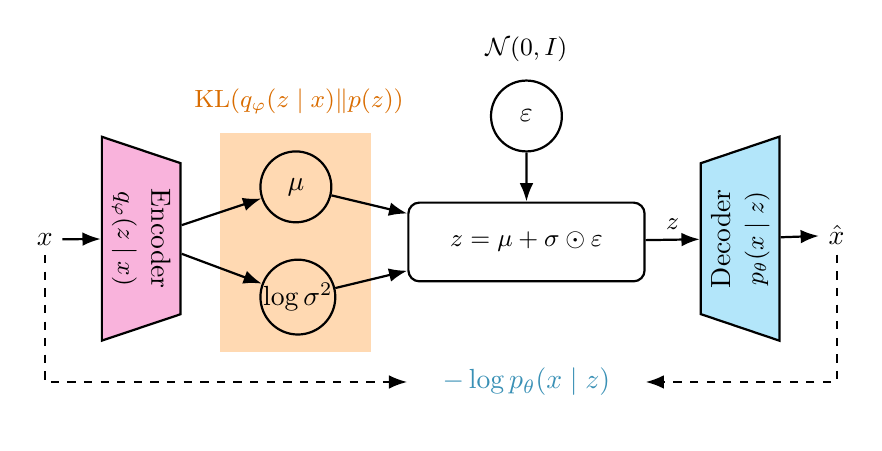
\begin{tikzpicture}[
    >=Latex,
    node distance=16mm and 8mm,
    box/.style={draw, rounded corners, thick, minimum width=30mm, minimum height=10mm, align=center},
    trap/.style={
        draw, thick,
        trapezium,
        trapezium stretches=true,
        minimum width=26mm,
        minimum height=10mm,
        align=center
    },
    var/.style={draw, circle, thick, minimum size=9mm, inner sep=0pt},
    small/.style={font=\small},
]

% encoder
\node[] (x) {$x$};
\node[trap, right=10mm of x,yshift=11.5mm,
      trapezium left angle=75,
      trapezium right angle=75,rotate=-90,fill=magenta!30] (enc)
      {Encoder\\\small $q_\varphi(z\mid x)$};
\draw[fill=orange!30,draw=none] ($(enc.east)+(2.92,-0.3)$) rectangle ($(enc.west)+(1,0.2)$);
\node[right=15.5mm of x,yshift=17.5mm,orange!85!black] {\small$\mathrm{KL}(q_\varphi(z\mid x)\|p(z))$};
\node[var, right=15mm of enc, yshift=18mm] (mu) {$\mu$};
\node[var, right=15mm of enc, yshift=4mm] (logv) {$\log\sigma^2$};
\draw[->, thick] (x) -- (enc);
\draw[->, thick] (enc) -- (mu);
\draw[->, thick] (enc) -- (logv);

% reparameterization
\node[var, right=20mm of mu, yshift=9mm] (eps) {$\varepsilon$};
\node[small, above=1mm of eps] {$\mathcal N(0,I)$};
\node[box, right=9mm of logv,yshift=7mm] (reparam) {\small $z=\mu+\sigma\odot\varepsilon$};
\draw[->, thick] (mu) -- (reparam);
\draw[->, thick] (logv) -- (reparam);
\draw[->, thick] (eps) -- (reparam);

% decoder
\node[trap, right=12mm of reparam,yshift=-11mm,
      trapezium left angle=75,
      trapezium right angle=75,rotate=90,fill=cyan!30] (dec)
      {Decoder\\\small $p_\theta(x\mid z)$};
\node[right=10mm of dec,yshift=-11mm] (xhat) {$\hat{x}$};
\draw[->, thick,yshift=-9mm] (reparam) -- node[above, small] {$z$} (dec);
\draw[->, thick] (dec) -- (xhat);

% losses
\node[box, below=24mm of eps, minimum width=30mm,cyan!70!black,draw=white] (loss) {
$-\log p_\theta(x\mid z)$};

\draw[->, thick,dashed] (xhat.south) |- (loss.east);
\draw[->, thick,dashed] (x.south) |- (loss.west);
% \draw[->, thick] (mu.south) |- (loss.north);
% \draw[->, thick] (logv.south) |- (loss.north);

\end{tikzpicture}
\end{document}


